\documentclass[tikz,border=6pt]{standalone}
\usepackage{amsmath}
\usetikzlibrary{decorations.pathreplacing}

\definecolor{matred}{RGB}{192,0,0}
\definecolor{toppeach}{RGB}{244,177,131}
\definecolor{laborfill}{RGB}{251,229,214}
\definecolor{capitalfill}{RGB}{248,203,173}
\definecolor{profitgray}{RGB}{166,166,166}

\begin{document}
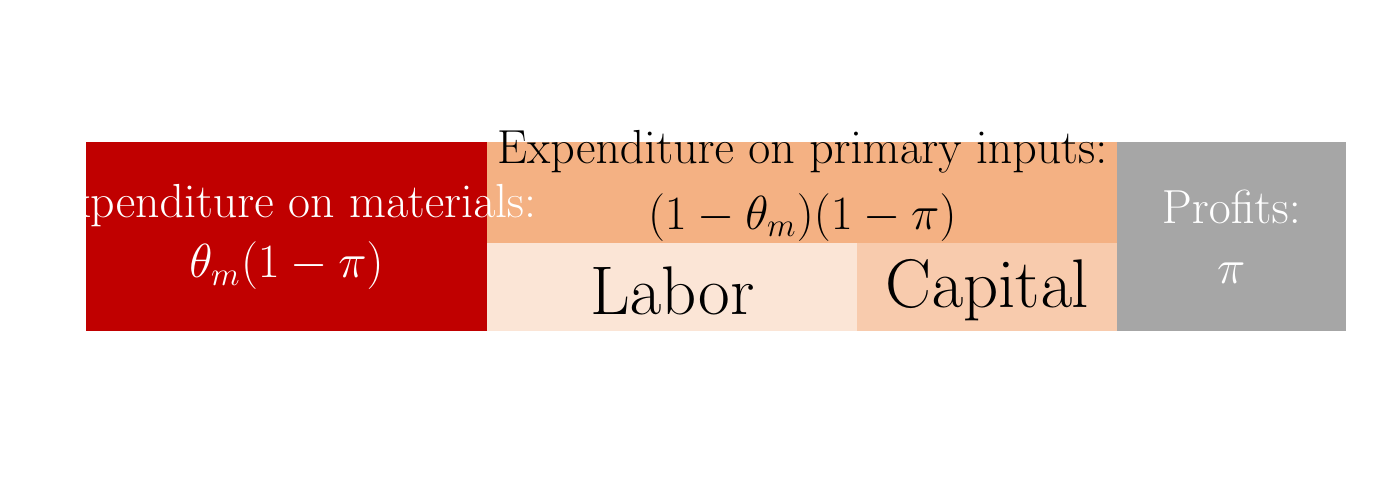
\begin{tikzpicture}[x=1cm,y=1cm]
  \def\W{16}
  \def\H{2.4}
  \def\TopH{1.28}
  \def\BottomH{1.12}
  \def\MatW{5.1}
  \def\PrimaryW{8.0}
  \def\ProfitW{2.9}
  \def\LaborW{4.7}
  \def\CapitalW{3.3}

  \fill[matred] (0,0) rectangle (\MatW,\H);
  \fill[toppeach] (\MatW,\BottomH) rectangle (\MatW+\PrimaryW,\H);
  \fill[laborfill] (\MatW,0) rectangle (\MatW+\LaborW,\BottomH);
  \fill[capitalfill] (\MatW+\LaborW,0) rectangle (\MatW+\PrimaryW, \BottomH);
  \fill[profitgray] (\MatW+\PrimaryW,0) rectangle (\W,\H);

  \node[white,align=center,font=\fontsize{17}{20}\selectfont] at (2.55,1.2)
    {Expenditure on materials:\\[2pt]$\theta_m(1-\pi)$};

  \node[align=center,font=\fontsize{18}{22}\selectfont] at (\MatW+0.5*\PrimaryW,1.85)
    {Expenditure on primary inputs:\\[2pt]$(1-\theta_m)(1-\pi)$};

  \node[font=\fontsize{24}{28}\selectfont] at (\MatW+0.5*\LaborW,0.52) {Labor};
  \node[font=\fontsize{24}{28}\selectfont] at (\MatW+\LaborW+0.5*\CapitalW,0.52) {Capital};

  \node[white,align=center,font=\fontsize{17}{20}\selectfont] at (\MatW+\PrimaryW+0.5*\ProfitW,1.2)
    {Profits:\\[2pt]$\pi$};

  \draw[white,decorate,decoration={brace,amplitude=7pt},line width=0.7pt]
    (0,\H+0.12) -- (\W,\H+0.12)
    node[midway,yshift=0.95cm,font=\fontsize{18}{22}\selectfont] {Total Gross Output $=1$};

  \draw[white,decorate,decoration={brace,mirror,amplitude=7pt},line width=0.7pt]
    (\MatW,-0.12) -- (\W,-0.12)
    node[midway,yshift=-0.95cm,font=\fontsize{17}{21}\selectfont]
    {Total Value Added $= 1-\theta_m(1-\pi)$};
\end{tikzpicture}
\end{document}
